\documentclass[../main.tex]{subfiles}
\graphicspath{{\subfix{../imgs/}}}
\begin{document}
\newpage

\chapter{Project Architecture}

\section{Design Concerns and Choices}
The task proposed in this project necessitated many early design choices that greatly affected the choice of software and libraries that would be used for the remainder of the project. Some of these concerns included:

\begin{itemize}

    \item\textbf{Input Data Type} — For the task of Music Generation we can choose to work with 1) \textit{real-time audio} or 2) \textit{a symbolic representation of the music}, in a format such as MIDI. The choice of input greatly affects the model architecture, its output, as well the it's overall speed. Furthermore the choice of data format informs the choice of dataset, and it is critical to use data of a high quality
    
    \item \textbf{The Model Environment} — Given the project's aim to create a live, improvisation centric system, we first require an environment/software that is able to easily:
    
    \begin{enumerate}
        \item Record live auditory information
        \item Transform it into a format acceptable to the model
        \item Trigger model inference
        \item Generate musical output given the model's output
    \end{enumerate}
    
    Additionally, for the system to be accessible to non-technical musicians, it would ideally support some form of visual GUI that makes it relatively easy to use and learn, while abstracting away much of the core logic in the program.
    
    
    \item \textbf{Separating model training from the performance environment} — Given the above, the model would likely have to live in an environment separate from the one it was trained in. Therefore the model must be flexible and support being exported and deployed to the environment of choice. 

    \item \textbf{Model Size} — Our model had to balance between being large enough to extract meaningful information from large amounts of sequential data, while also being small enough such that inference could still be relatively quickly. 
    
\end{itemize}

Taking the above concerns and the problem statement into account, I made several design choices:

\begin{enumerate}

    \item\textbf{Input Data Type} - To minimize the amount of processing required, I explicitly decided to use the midi encoding proposed by Oore et. al\cite{oore:1} While this greatly lessens the processing requirement of the model itself, it places the onus of extracting a meaningful stream of MIDI data from the model environment.

    \item \textbf{The Model Environment} - The model's performance environment is constructed in Max/MSP \cite{max/msp}. Max/MSP — also known as Max — is a visual programming paradigm for music and multimedia developed by Cycling '74. It provides a graphical interface for creating and manipulating audio, video, and other multimedia content and is widely used in the fields of music composition, live performance, sound design, and interactive multimedia art. It is easy to use, highly optimized as an audio processing unit, and has an assortment of pre-built modules that directly address our needs, like a pitch-tracking module. 

    Furthermore, Max/MSP features an internal Node.js runtime engine that can run and interact with custom Javascript scripts. With the full flexibility of Javascript at our disposal within Max/MSP, I have opted to use the Node.js runtime to create an Improvisor class that houses our transformer model and serves as the interface between our model and Max/MSP. All custom is currently being written in Typescript before being compiled into Javascript.

    \item \textbf{Choice of Framework} - The most popular ML frameworks available today are PyTorch and Tensorflow, both of which leverage Python as the main language to train ML models. While PyTorch is reportedly easier to use and prototype models with, I have chose to use Tensorflow as my Machine learning library of choice, as it has a Javascript port, \textit{Tensorflow.js}, that can run models built and compiled with the regular Tensorflow package and Python. This would effectively allow me to train and build my model in a separate Python environment, and then load it within the Node.js runtime housed within Max.
\end{enumerate}

While the source code for the Music Transformer paper by Google has not yet been released, I found a 3rd party implementation of the paper by a PHD researcher {INSERT} on Github. While this implementation was helpful in understanding the various components of the Transformer, my own implementation differs significantly.

\chapter{Data}

\section{Choice of Dataset}
For the purpose of this project, I decided to use the MAESTRO dataset\cite{hawthorne:1} used by Huang et.al \cite{Huang:1} during their attempt to build a modified transformer model for long-context music generation. Put together by the same team, MAESTRO (MIDI and Audio Edited for Synchronous TRacks and Organization) is a dataset composed of about 200 hours of virtuosic piano performances captured with fine alignment (~3 ms) between note labels and audio waveforms. The dataset is made available by Google LLC under a Creative Commons Attribution Non-Commercial Share-Alike 4.0 (CC BY-NC-SA 4.0) license.

While there are several other datasets of paired piano audio and MIDI have been that published previously and have enabled significant advances in MIR tasks, I choose to use the MAESTRO dataset for several reasons. First, MAESTRO is around an order of magnitude larger than most other similar datasets, as shown making it a perfect choice for training transformer models that notoriously require a lot of data. Second, the quality of recorded midi performances in the MIDI dataset is extremely high, having been collected from several annual runs of the International Piano e-competition {CITE}. Virtuoso pianists perform on Yamaha Disklaviers: concert quality acoustic grand pianos that utilize an integrated high-precision MIDI capture and playback system. The recorded data is of sufficient fidelity to allow the audition stage of the competition to be judged remotely by listening to contestant performances reproduced over the wire on another Disklavier instrument.  

Below is information collected about other similar datasets that were considered for this task by Hawthorne et.al\cite{hawthorne:1}:

\begin{figure}[hp]
    \centering
    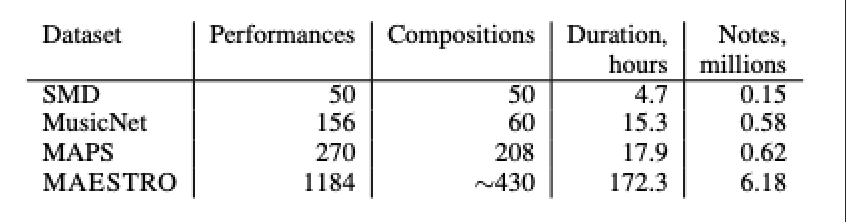
\includegraphics[width=1\textwidth]{imgs/maestro_comparison.png}
    \caption{Comparing Maestro to other datasets (Taken directly from Hawthorne et al.)}
    \label{table:maestro_comparison}
\end{figure}

\textbf{MusicNet} (Thickstun et al., 2017) contains recordings of human performances, but separately sourced scores. As discussed in Hawthorne et al. (2018), the alignment between audio and score is not fully accurate. One advantage of MusicNet is that it contains instruments other than piano (not counted in table 2) and a wider variety of recording environments, making it more flexible for ML tasks that deal directly with audio. 

\textbf{MAPS} (Emiya et al., 2010) contains Disklavier recordings like MAESTRO and synthesized audio created from MIDI files that were originally entered via sequencer. The synthesized audio makes up a large fraction of the MAPS dataset, which implies that many of the performances are not as expressive as the MAESTRO tracks captured from live performances, making it less attractive for the task of musical improvisation.

\textbf{Saarland Music Data (SMD)} (Muller et al., 2011) is very similar to MAESTRO in that it contains recordings and aligned MIDI of human performances on a Disklavier, but is far smaller than the MAESTRO dataset

\section{Dataset Analysis}

\begin{figure}[hp]
    \centering
    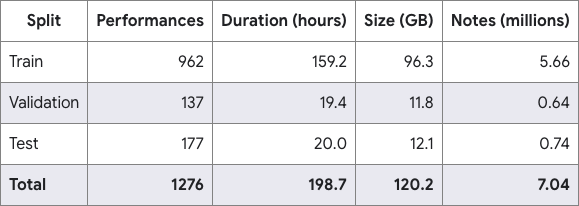
\includegraphics[width=1\textwidth]{imgs/maestro_split.png}
    \caption{Split from the Maestro Dataset v3.0.0 (From \nolinkurl{https://magenta.tensorflow.org/datasets/maestro}.)}
    \label{table:maestro_split}
\end{figure}

The figure above gives us some brief statistics about the data set as well as details about a proposed train, validation and test split. Hawthorne et. al note that this split was proposed so that: 

\begin{enumerate}
    \item No composition should appear in more than one split
    \item Train/validation/test should make up roughly 80/10/10 percent of the dataset (in time) respectively and that the validation and test splits should contain a variety of compositions
    \item Extremely popular compositions performed by many performers should be placed in the training split.
\end{enumerate} 

They also note that these proportions should be true globally and also within each composer's corpus of performed work. However, they also note that maintaining these proportions however, is not always possible because some composers have too
few compositions in the dataset.

TODO: Histograms of num pieces in each split by composer (can be viewed as a specific style) and by key (a specific pitch distribution)

TODO: Histograms of num pieces in each split by composer, weighted by duration

\section{MIDI Encoding and Input Representation}

The MIDI protocol covers a wide variety of message types, which raises a new challenge for our input representation. Hence, we adopt a sparse, MIDI-like representation from Oore et al. \cite {oore:1} that specifically encodes information about pitch and time in an event-based manner. The vocabulary of this encoding consists of 128 NOTE-ON events, 128 NOTE-OFFs, 100 TIME-SHIFTs allowing for expressive timing at 10ms (specifically from the MAESTRO dataset) and 32 VELOCITY bins for expressive dynamics, as shown in Figure \ref{fig:fig3}. 

\begin{figure}[htpb]
    \centering
    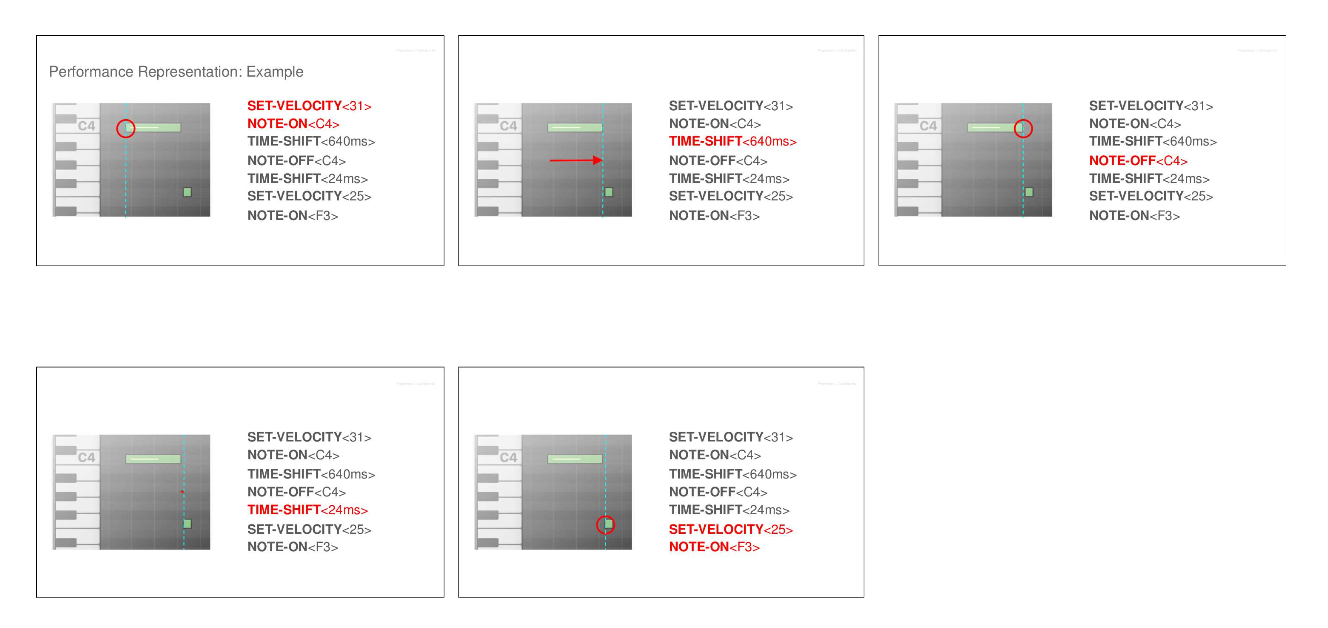
\includegraphics[width=1\textwidth]{imgs/midi_encoding.png}
    \caption{An illustration from Oore et al. of how a MIDI sequence is converted into a sequence of commands in our event vocabulary. Note: an arbitrary number of events can in principle occur between two time shifts.}
    \label{fig:fig3}
\end{figure}

The implementation of the MIDI encoding process was outsourced to a 3rd party library \textbf{midi-neural-preprocessor}, developed by {INSERT NAME}, the same researcher who attempted to implement the Google Paper on long context music-generation with Transofrmers. To process all of the MIDI files in the MAESTRO dataset, I wrote a Preprocessor class that employs multi-threading to encode each MIDI file and save it in a binary format.

% FROM PAPER As position in sequence no longer corresponds to time, a priori it is not obvious that relative attention should work as well with such a representation. However, we will show in Section 4.2 that it does improve perplexity and sample quality over strong baselines.

I also conducted a statistical analysis of event sequences across all the MIDI files, gleaning some interesting results.

TODO: Discuss Statistics for event sequences by Split (Average, length, max, min, as well events that do not appear at all or appear overwhelmingly across sequences)


\section{Building an input pipeline in Tensorflow}
Given that I was  dealing with a substantial amount of sequential data across thousands of files it was of paramount importance to experiment with different data pipelines and consider which was best suited for me given the limited compute resources on hand. While the raw encoded sequences themselves could all fit into memory, it is important to note that the training examples for the model are constructed by grabbing fixed length event sequence windows from the sequence, with a stride of 1. This results in an explosion of our data's memory footprint, illustrated below. 

TODO: Provide brief diagram showing size of raw midi -> how many batches we actually extract given a window of size L and the resulting size of all the extracted training examples.

\subsection{The BaseDataset class}
- Parent class for various dataset implementations. Reads in and stores all the paths to the encoded midi binaries, while also filtering out some files based on minimum duration, or minimum event sequence length

\subsection{The TestDataset class}
- Subclasses BaseDataset. Built to first generate simple test sequences in memory to evaulate early models
1) Can generate major scale midi numbers across all keys, useful metric to see if the Transformer could first learn very basic data

2) Retrieves all the training examples from just one file, separating them into an 80/10/10 training , validation and test split that is shuffled around the file

3) Retrieves all files to attempt construction of an in-memory dataset

4) V2 of in-memory dataset that is optimized with numpy operations and integer types with a smaller memory footprint. Significant improvements, but not enough to load all data into memory

\subsection{The SampledDataset class}

\subsection{The SequenceDataset class}

\subsection{The MappedDataset class}

\subsection{Analyzing GPU Profiles}


\subsection{Thinking about the model}
Given our desire to train a robust model that is able to function in real-time, the size of our model needed to simultaneously be small enough such that inference did not take extremely long, while also being large enough to encode the large amount of midi information being fed to it. For this purpose I decided to work with an architecture that is very similar to the baseline transformer architecture proposed in Vaswani et. al\cite{Vaswani:1}.
\end{document}
